\section{わかるらんど}

\subsection{ユーザインタフェース}

図\ref{dashboard}図\ref{console}\footnote{タイトル ブラックジャックによろしく\newline 著作者名 佐藤秀峰\newline サイト名 漫画 on web}はわかるらんどのスクリーンショットである.
ユーザインタフェースは,ダッシュボード,投稿画面の2つからなる.
ダッシュボードと投稿画面はいずれも単一の画面で,上部のボタンで切り替えて利用する.
ダッシュボードには指定した情報を表示するウィジェット(図\ref{widget})を格子状に並べることができる.

ウィジェットには人間の感情や現在の状況を表示するwakariウィジェットと,センサ情報などの数値を表示するdataウィジェットの2種類がある.
ウィジェットのバックグラウンドには人/物/現象の画像を表示し,その上に情報をオーバーレイで表示する.
情報はリアルタイムに更新が反映され,最新の情報のみを表示する.

投稿画面ではユーザとしてダッシュボードに投稿を行うことができる.
ユーザの投稿は「スタンプ」をクリックすることで行う.
スタンプは,
\begin{itemize}
\item わかるらんどのテキストをスタンプ化する機能を使う
\item 画像のURL
\end{itemize}
の2つの方法で一覧に追加することができる.
また,スタンプ投稿時にクリックの長さを変えることで,ダッシュボードにスタンプを表示する時間の変更が可能である.

\begin{figure}[h]
\centering
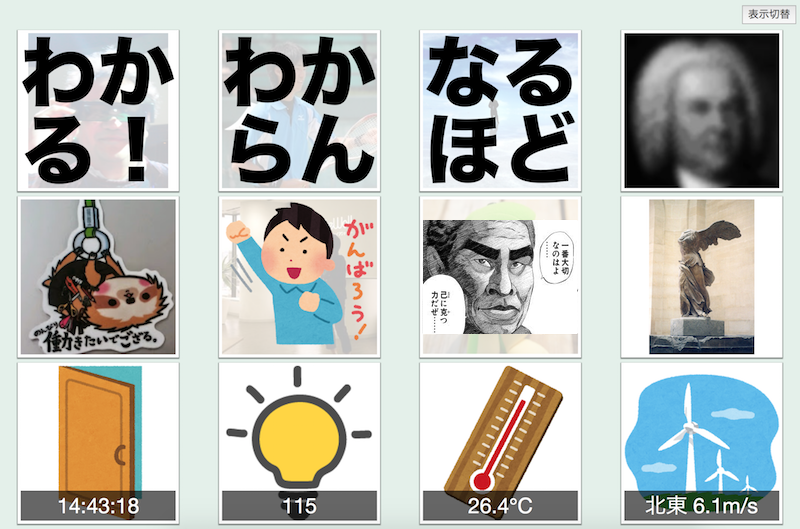
\includegraphics[width=7cm]{images/dashboard.png}
\caption{わかるらんどのダッシュボード}
\label{dashboard}
\end{figure}

\begin{figure}[h]
\centering
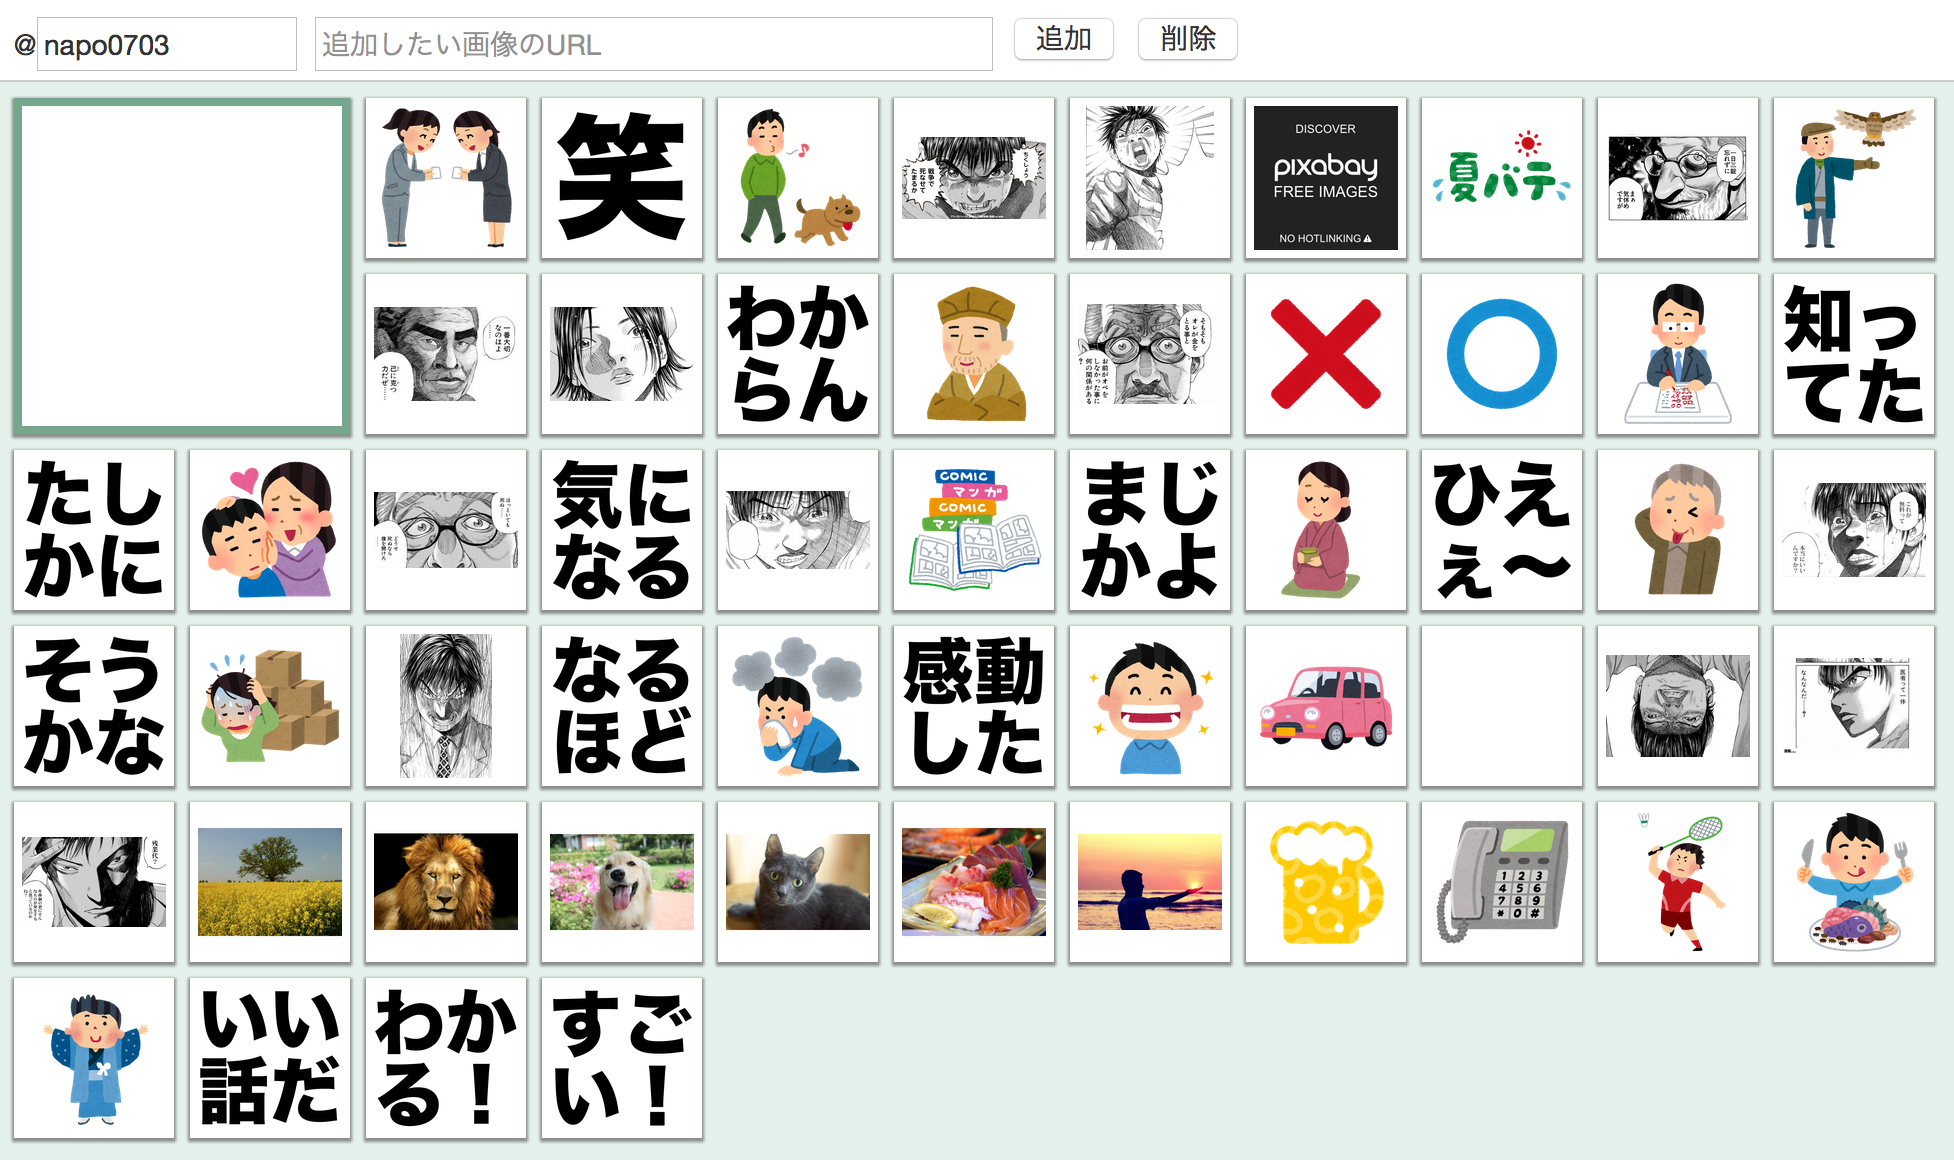
\includegraphics[width=7cm]{images/console.png}
\caption{わかるらんどの投稿画面}
\label{console}
\end{figure}

\begin{figure}[h]
\centering

\includegraphics[width=7cm]{images/widget.png}
\caption{wakariウィジェット(左)とdataウィジェット(右)}
\label{widget}
\end{figure}

\subsection{利用例}

\subsubsection{投稿する感情や現在の状況の例}

わかるらんどで表示できる感情や現在の状況の例を示す.

\begin{itemize}
\item 「わかる」「わからない」「そうだね」等の相づち
\item 「仕事中」「寝てる」等の現在やっていること
\item 現在位置
\item 食べたものや現在いる場所の写真
\item ニュースや天気予報
\item 温度や明るさ等のセンサの値
\item Webカメラの映像
\item トイレの空き状況
\item メールの未読件数

数値,文字列,イラスト,写真,動画など非常に幅広い表現が可能である.

\end{itemize}

\subsubsection{発表や講義での利用例}

図\ref{discussion}は講義や発表での利用例である.
これをサブスクリーンに表示することで,他の参加者の感情を把握したり登壇者が聴衆の反応を見ながら発表をしたりすることができる.
また図\ref{vote}のようにアンケートを取ったり,図\ref{rescue}のように「寒い」「トイレに行きたい」「お腹が痛い」など,
口頭では伝えにくい感情や議論とは関係のない通知を話の腰を折ることなく周囲それとなくに伝えることもできる.

\begin{figure}[h]
\centering
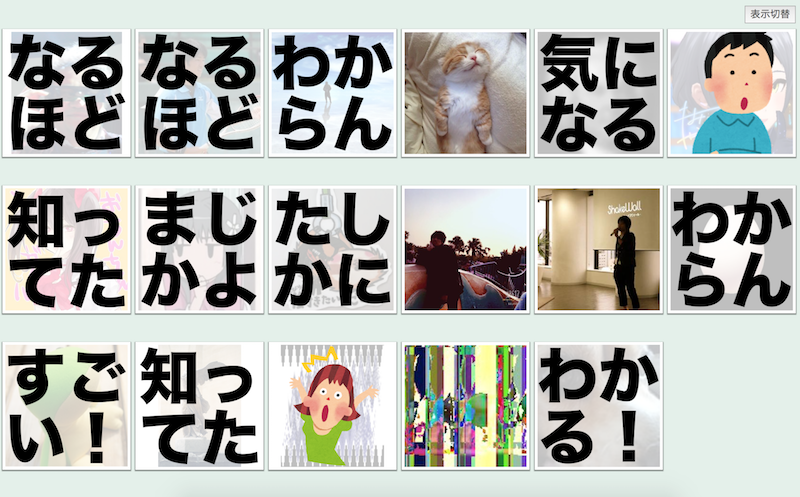
\includegraphics[width=7cm]{images/discussion.png}
\caption{会議での利用}
\label{discussion}
\end{figure}

\begin{figure}[h]
\centering
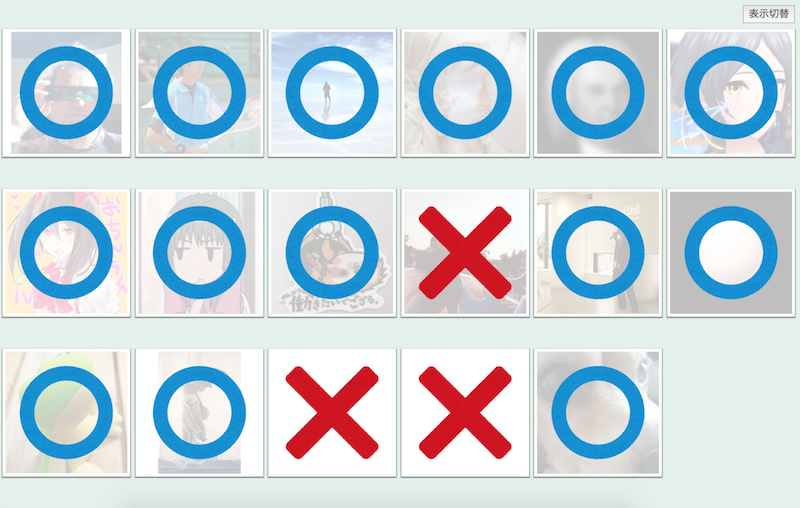
\includegraphics[width=7cm]{images/vote.png}
\caption{アンケートとしての利用}
\label{vote}
\end{figure}

\begin{figure}[h]
\centering
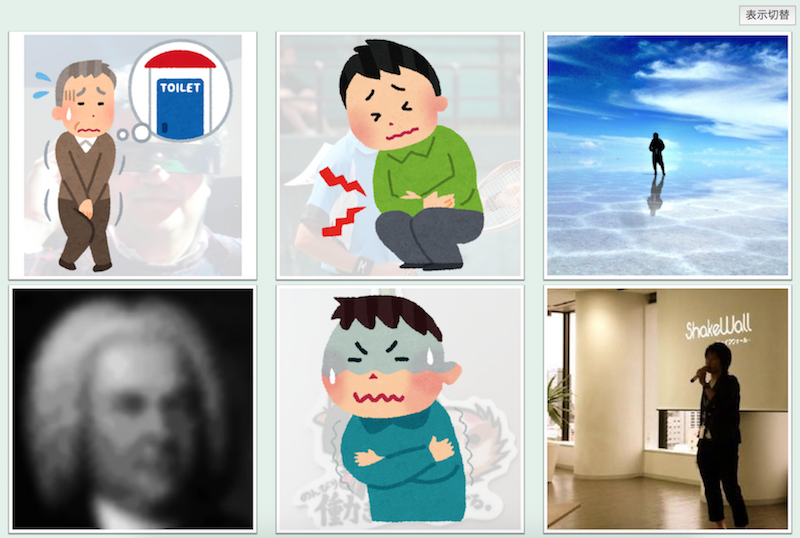
\includegraphics[width=7cm]{images/rescue.png}
\caption{言い出しにくいことを伝える}
\label{rescue}
\end{figure}

\subsubsection{センサ情報等の表示}

図\ref{sensors}は,明るさ,ドアが最後に開いた時間,気温,風速,天気,メール未読件数,株価,電力使用量を表示した例である.
センサの値やインターネット上の情報,コンピュータの情報などをひと目で把握することができる.

\begin{figure}[h]
\centering
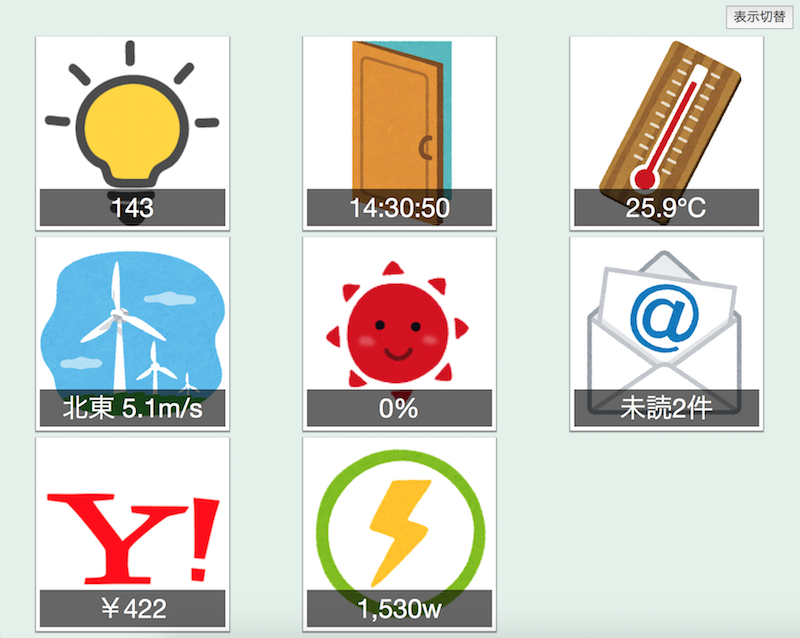
\includegraphics[width=7cm]{images/sensors.png}
\caption{センサやWebの情報を表示}
\label{sensors}
\end{figure}

\subsubsection{家庭内サイネージ}

図\ref{home}は家庭での利用例である.
左上の「夕食は家で食べるか」という問いかけに対して返答したり,「勤務中である」「渋谷にいる」といった現在の状況を表示することもできる.

また,ペットなど人間以外にセンサを取り付けて投稿させることも可能である.

\begin{figure}[h]
\centering
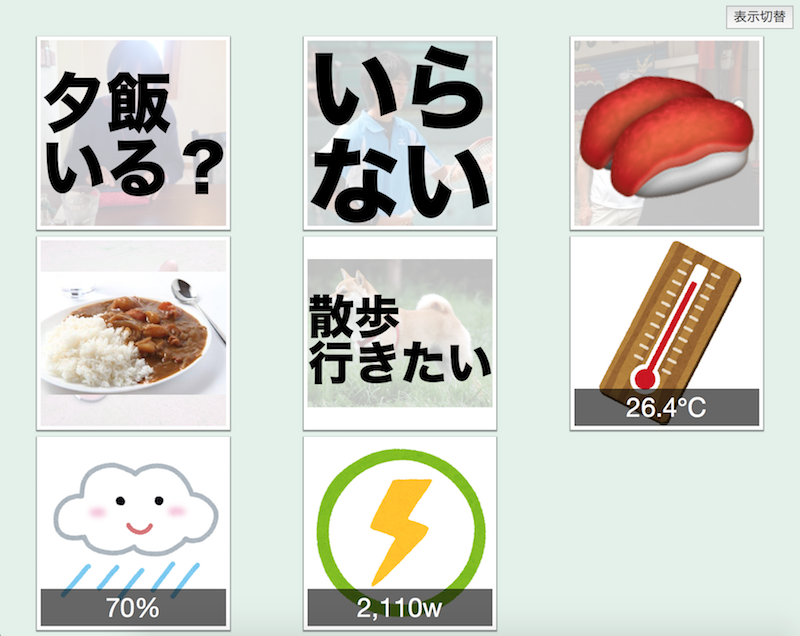
\includegraphics[width=7cm]{images/home.png}
\caption{家庭での利用}
\label{home}
\end{figure}